\section{Parameterized LLM Cost Model}
\label{sec:bench}

\subsection{Profile Interface}
OrbitLLM uses a profile table rather than a generic CPU-cycle cost. Each row contains model name, scale, quantization, context length, prefill tokens, decode tokens, prefill joules/token, decode joules/token, decode throughput, peak memory, and GPU power. We generated this table on a remote RTX 4090 24GB host using local copies of \texttt{Qwen3-1.7B}, \texttt{Qwen2.5-3B-Instruct}, and \texttt{Qwen3-8B}. The benchmark covers FP16, INT8, and INT4 inference at 1024, 2048, and 4096-token contexts with three runs per point; repeated runs are averaged before simulation. Replacing \texttt{results/profile\_anchor.csv} with another measured CSV automatically regenerates all scheduling results.

\subsection{Energy and Memory Surfaces}
\Cref{fig:energy} shows the measured separation between prefill and decode energy. The distinction matters because a long generation consumes more energy than a single averaged token coefficient would predict. \Cref{fig:memheat} shows peak memory over model scale and context length. This surface is used as a hard feasibility check in \cref{eq:c-mem}; if a task exceeds the memory ceiling, it cannot be assigned to \textsc{on}.

\begin{figure}[tb]
  \centering
  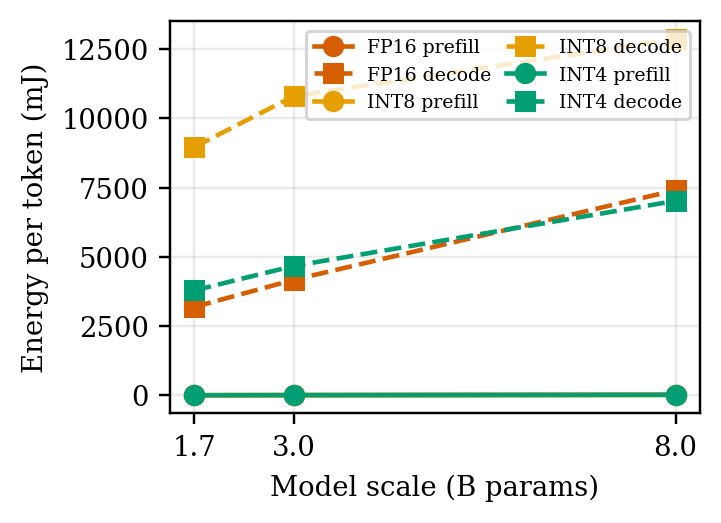
\includegraphics[width=\columnwidth]{figures/energy_per_token.png}
  \caption{Prefill and decode energy per token at 2048-token context. The scheduler indexes this surface when computing \cref{eq:eon}.}
  \label{fig:energy}
\end{figure}

\begin{figure}[tb]
  \centering
  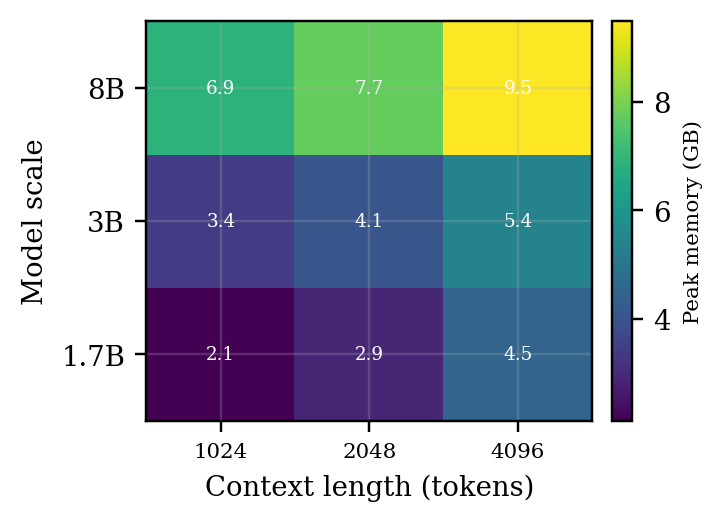
\includegraphics[width=\columnwidth]{figures/mem_heatmap.png}
  \caption{Peak memory for INT4 inference as a function of model scale and context length. The simulation uses a 16 GB on-board memory ceiling; all measured INT4 anchors fit below it.}
  \label{fig:memheat}
\end{figure}

\begin{table}[tb]
\centering
\caption{INT4 profile rows used by the reported simulation at 2048-token context. Energy is prefill/decode mJ per token, averaged over three runs.}
\label{tab:profile}
\small
\begin{tabular}{llccc}
\toprule
Model & Quant. & Tok/s & Energy/tok & Peak mem \\
\midrule
\ProfileRows
\bottomrule
\end{tabular}
\end{table}

\subsection{Why Parameterization Helps}
The purpose of this profile is not to claim flight-hardware performance. It is to make the scheduling assumption explicit and replaceable. Existing offloading models hide LLM behavior behind a scalar compute cost; OrbitLLM exposes the quantities that determine feasibility and value: memory fit, on-board latency, and token-level energy. The measured bitsandbytes INT8 path is not universally better than FP16 on this host, which reinforces the need to use hardware-specific profile rows rather than assumed quantization multipliers.
